% !TEX Root = ../proposal.tex

\section*{}
\subsection*{Motivation}  

% why go to asteroids

\begin{frame}[t]{Why send spacecraft to asteroids?}
    \begin{itemize}
        \item Some properties only available at the asteroid:
            \begin{itemize}
                \item High fidelity gravitational model
                \item Surface samples or return missions
            \end{itemize}
        \item Gain experience for future missions
            \begin{itemize}
                \item Weak gravitational field allows for less costly manuevers
                \item Asteroid tours for future deep-space human missions
            \end{itemize}
        \item Avoiding future impacts
            \begin{itemize}
                \item Local spacecraft can aid in ground based tracking
                \item Mitigation: Gravity tractors, kinetic impactors, solar sails etc.
            \end{itemize}
    \end{itemize}

\end{frame}

% Why use low thrust proplusion systems

\begin{frame} %-----------------------------%
\frametitle{Motivation - Low Thrust Transfers} % electric propulsion
\begin{itemize}
    \item Low-thrust orbital transfers
    \begin{itemize}
        \item Electric propulsion has increased in popularity

        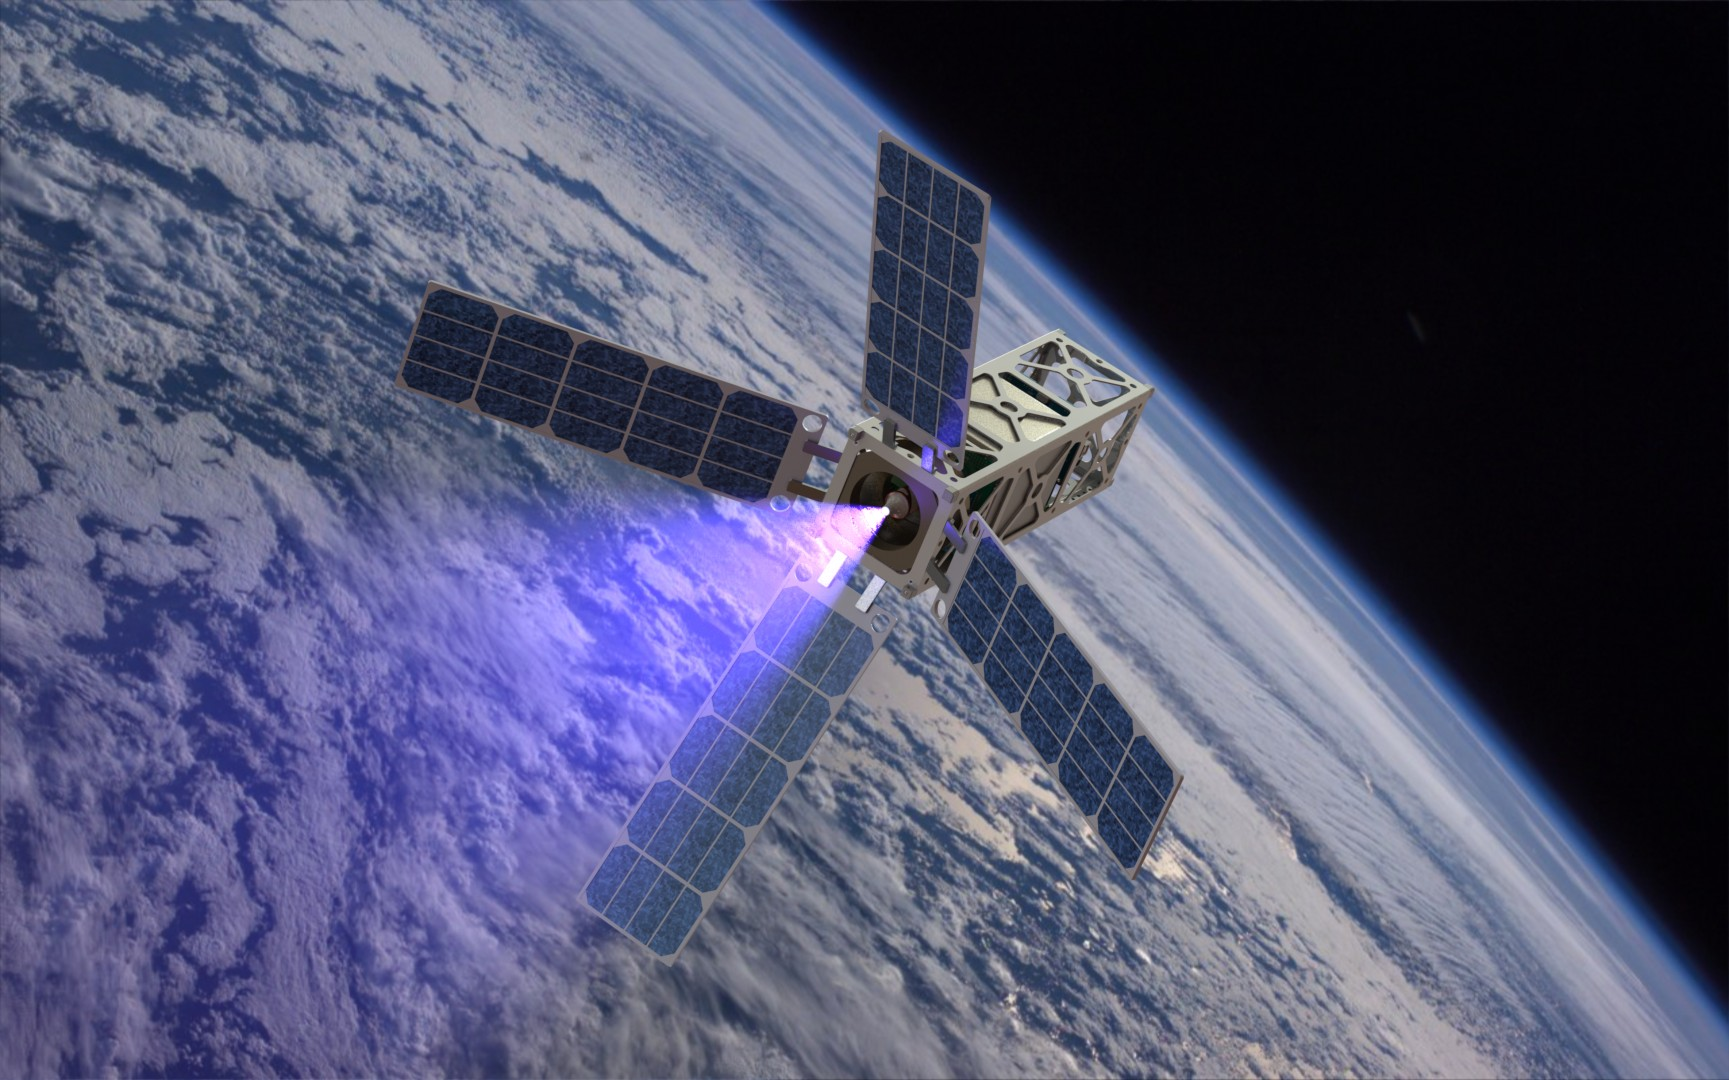
\includegraphics[height=0.3\textheight]{figures/2016AAS/patriot_plume.jpg}
        \hfill
        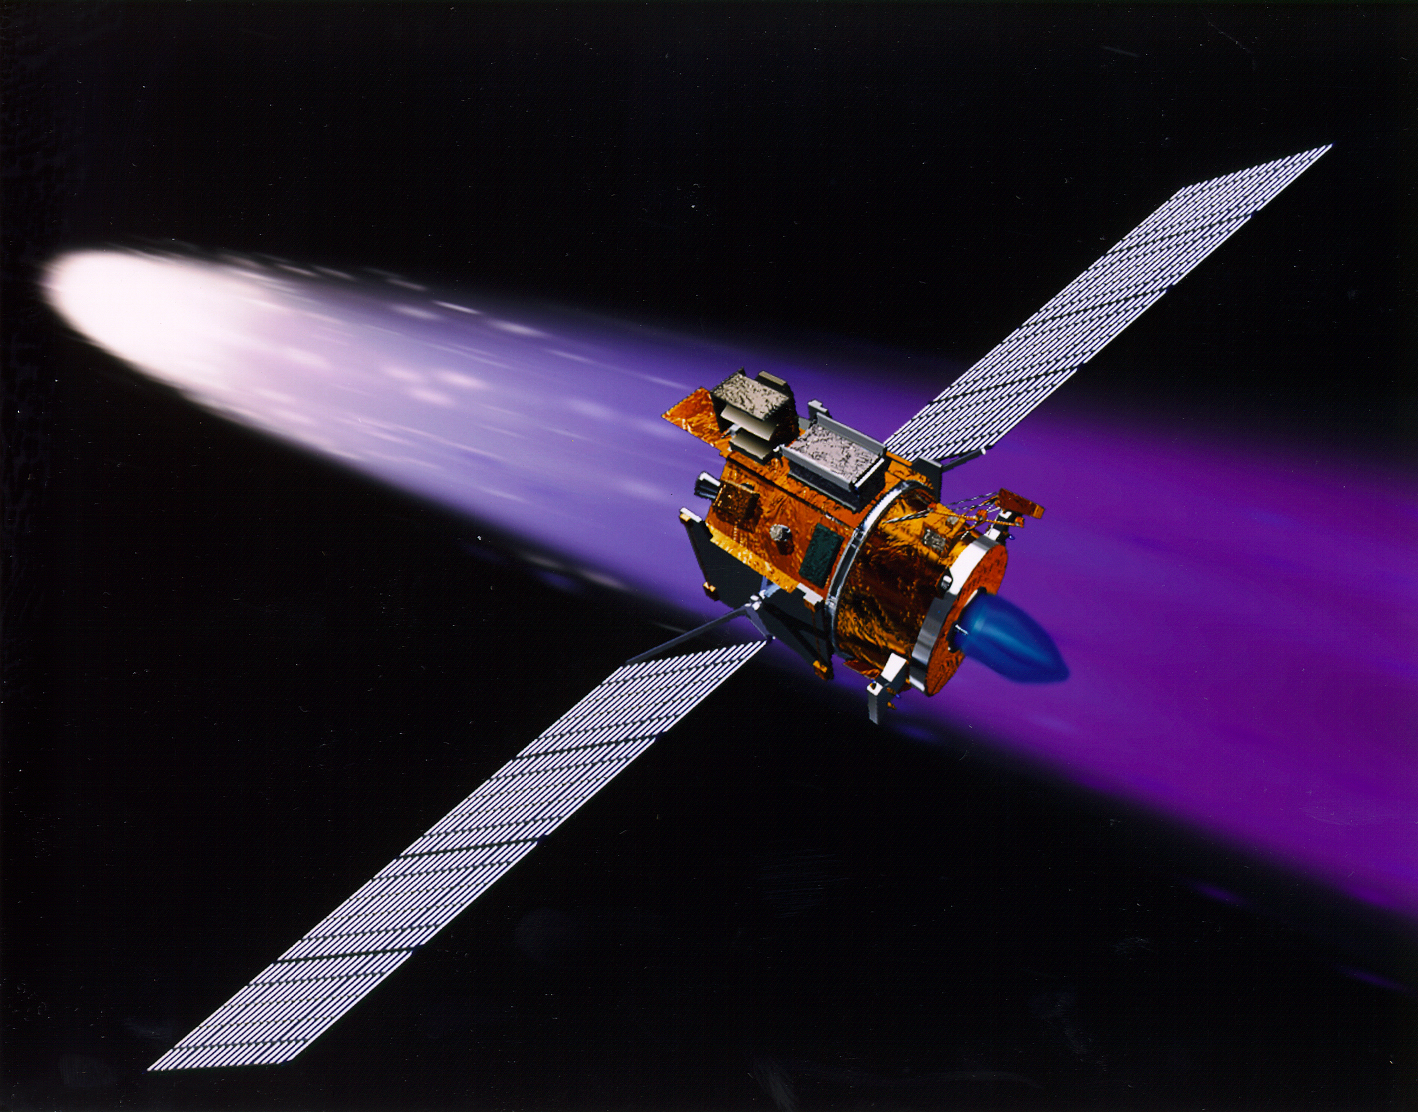
\includegraphics[height=0.3\textheight]{figures/2016AAS/deepspace1.jpg}
 
        \item Offers much higher specific impulse than chemical engines 
        
        \item Requires much longer operating periods for maneuvers 
        \item Small satellites with electric propulsion allows for new mission types
            \begin{itemize}
                \item Formation flight (distributed aperture sensing)
                \item On-orbit servicing
                \item Interplanetary swarms
            \end{itemize}
    \end{itemize}
\end{itemize}
\end{frame}   %-----------------------------%

\begin{frame} %-----------------------------%
\frametitle{Low-thrust vehicles} % electric propulsion
\begin{itemize}
    \item Low-thrust orbital transfers offer increased mission oportunities
    \begin{itemize}
        \item Electric propulsion is increasing in capability
        \item Offers much higher specific impulse than chemical engines 
        \item Requires much longer operating periods for maneuvers 
        \item Enables long duration missions with frequent thrusting
    \end{itemize}
\end{itemize}

\begin{center}
    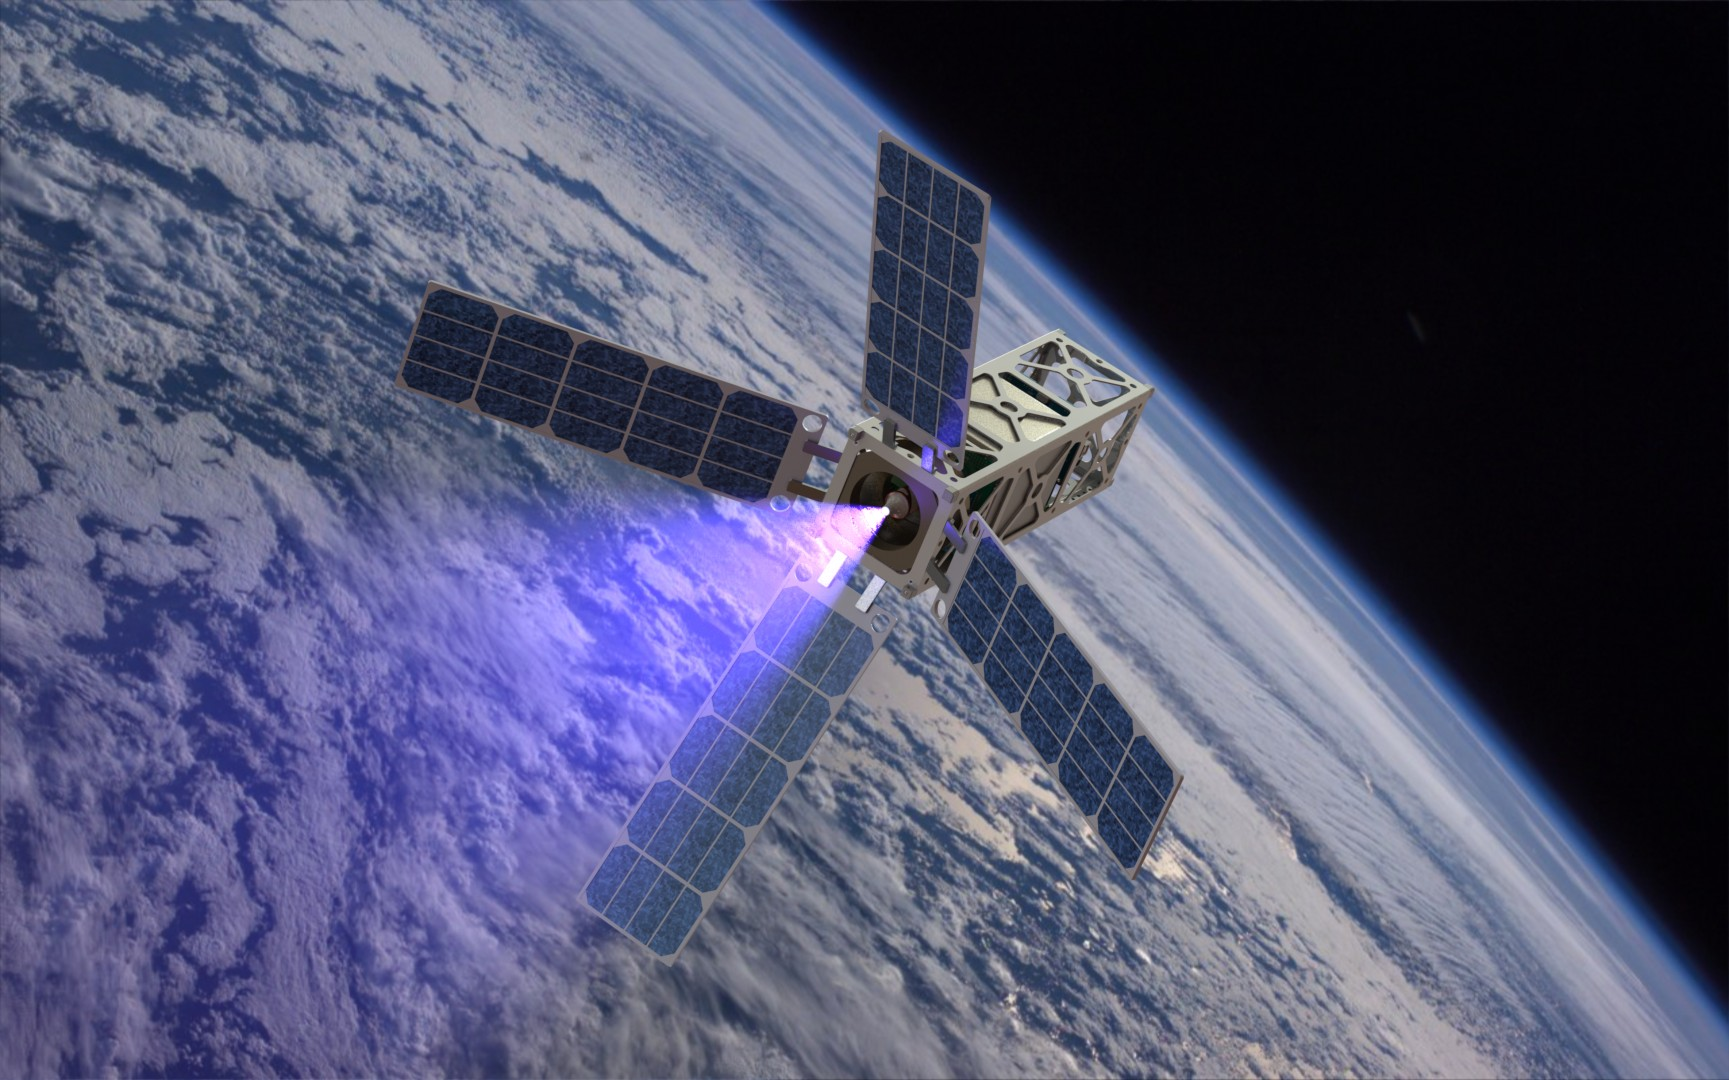
\includegraphics[width=0.5\textwidth,height=0.5\textheight,keepaspectratio]{figures/2016AAS/patriot_plume.jpg}
    ~
    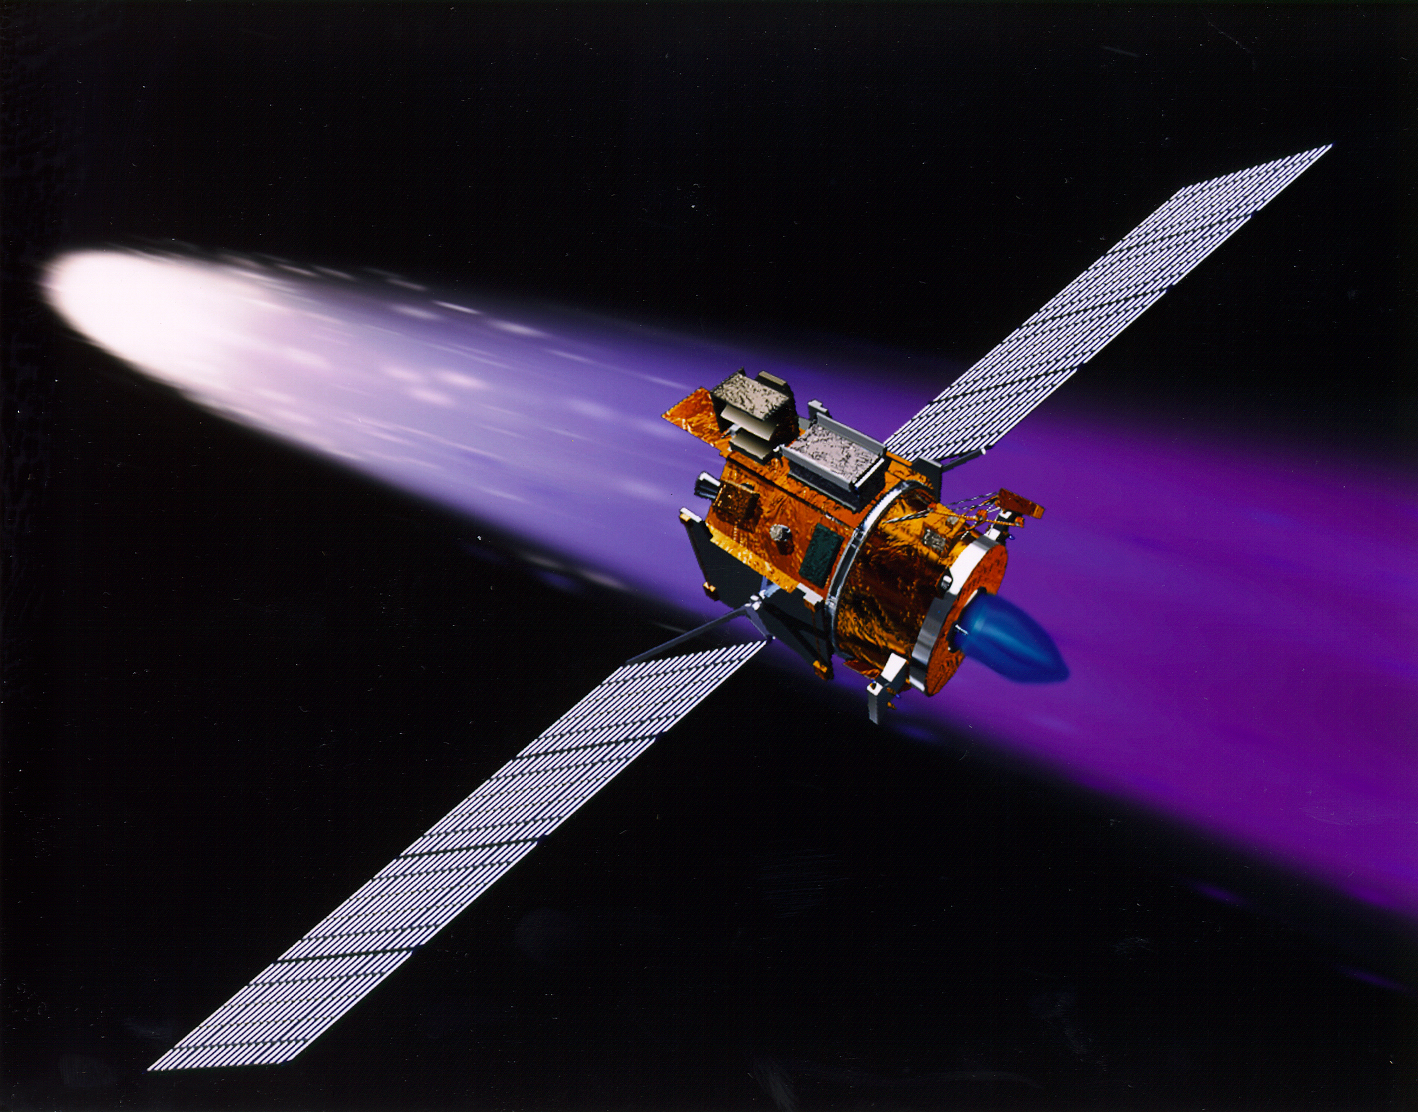
\includegraphics[width=0.5\textwidth,height=0.5\textheight,keepaspectratio]{figures/2016AAS/deepspace1.jpg}
\end{center}
\end{frame}   %-----------------------------%

\begin{frame}{Asteroids}
\begin{itemize}
    \item Science - insight into the early formation of the solar system
    \item Mining - vast quantities of useful materials
    \item Impact - high risk from hazardous near-Earth asteroids
\end{itemize}    

\begin{center}
    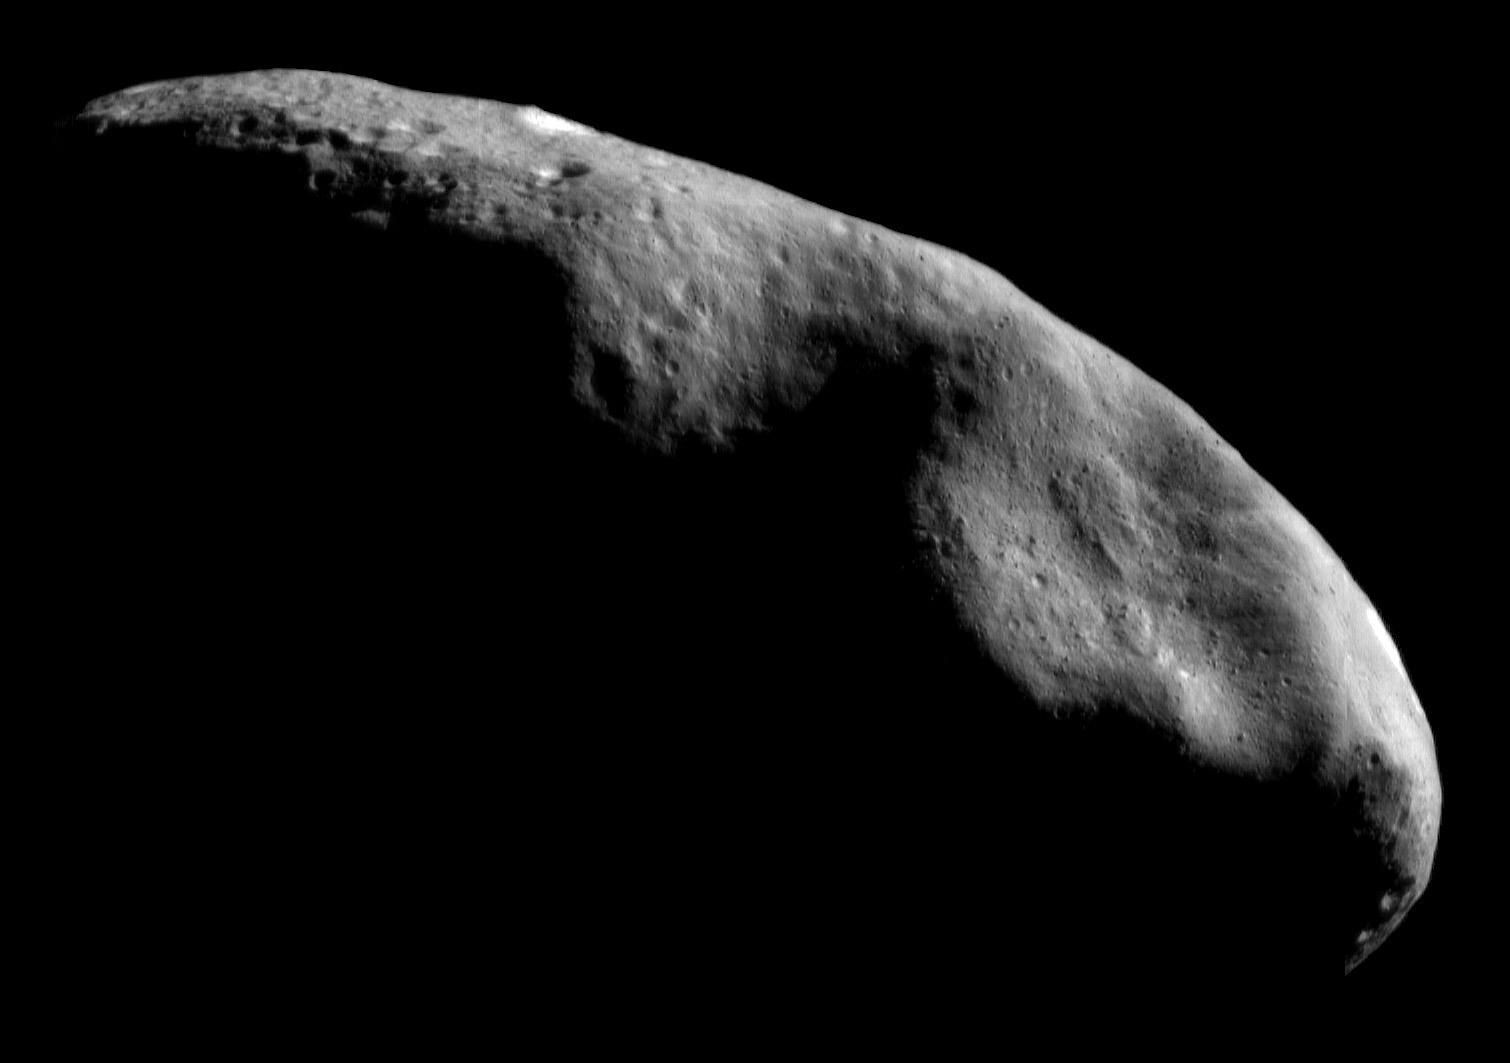
\includegraphics[width=0.5\textwidth,height=0.5\textheight,keepaspectratio]{figures/2016AAS/near_mos_20001203_full.jpg}
    ~
    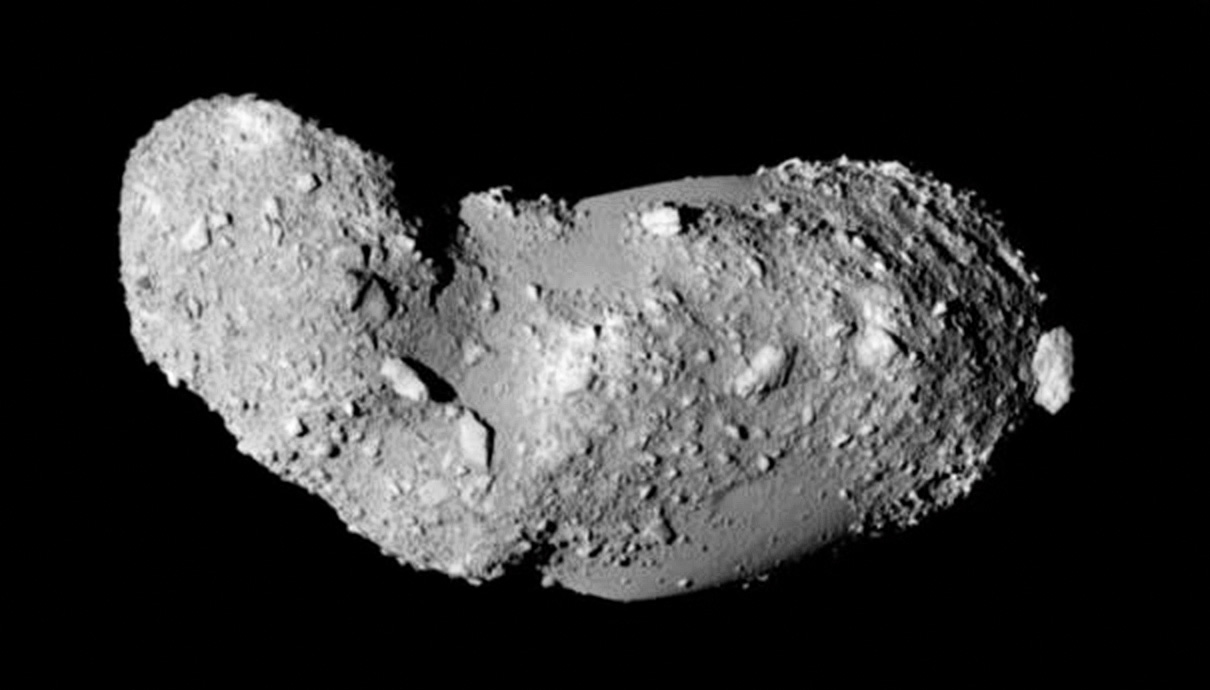
\includegraphics[width=0.5\textwidth,height=0.5\textheight,keepaspectratio]{figures/2016AAS/Itokawa8_hayabusa_1210.jpg}
\end{center}
\end{frame}

\begin{frame}[t]{Motivation} %-----------------------------%
\begin{itemize}
    \item Autonomous control of space vehicles is critical
    \begin{itemize}
        \item Avoid extensive planning and interaction by operators
        \item Ability to operate safely with system uncertainty 
        \item Independently navigate hazards and handle possible failures
    \end{itemize}
\end{itemize}
\visible<2->{
\begin{center}
    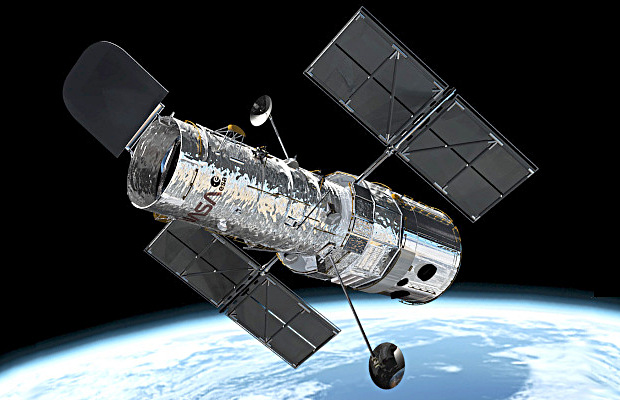
\includegraphics[width=0.5\textwidth,height=0.35\textheight,keepaspectratio]{figures/2016ACC/hubble.jpg}~
    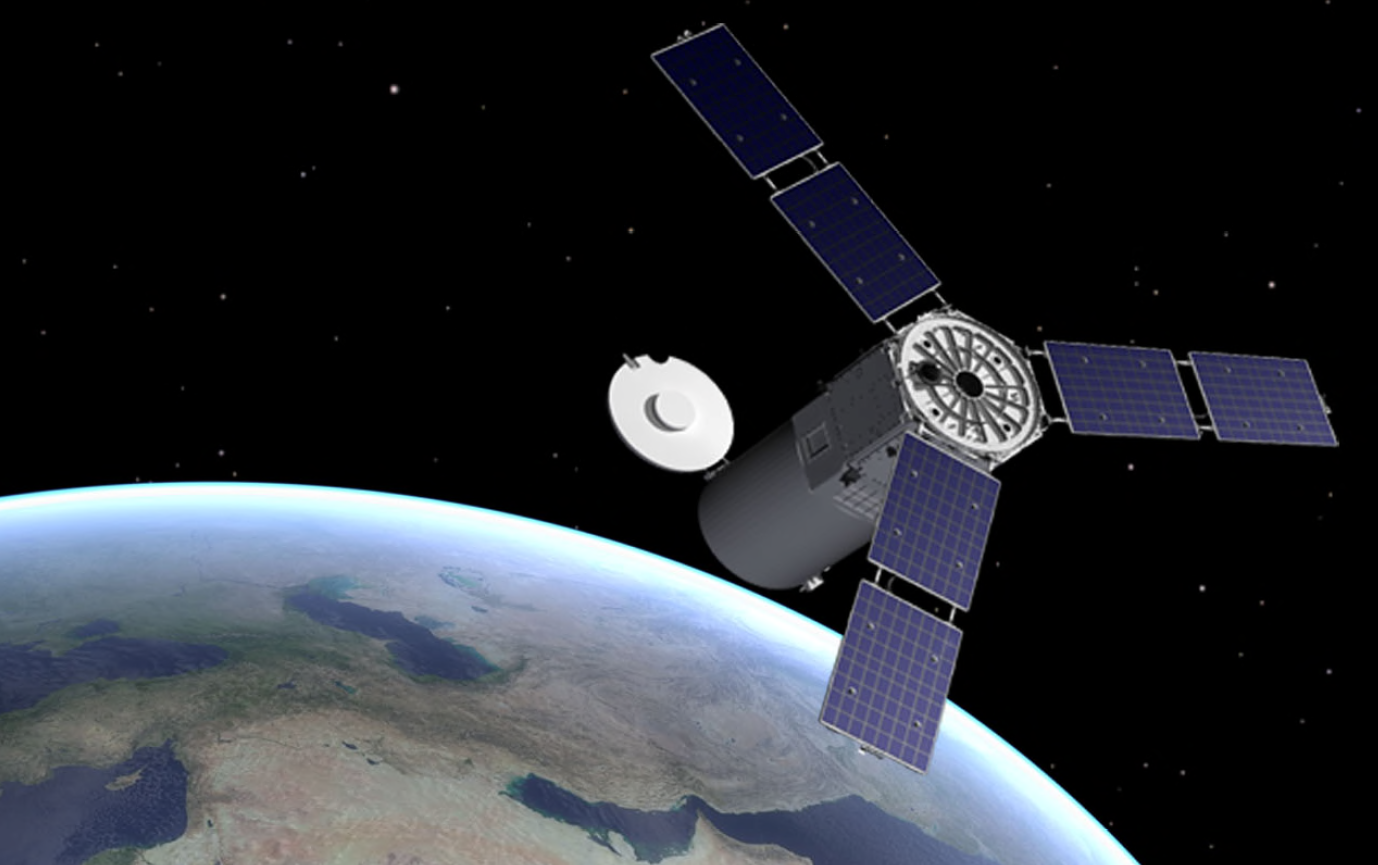
\includegraphics[width=0.5\textwidth,height=0.35\textheight,keepaspectratio]{figures/2016ACC/ors-1.png}
\end{center}
}
\end{frame}   %-----------------------------%